\graphicspath{{Chapter2/Chapter2Figs/}}

\chapter{TOR in ageing and age-related diseases}
\label{chap:TOR in ageing and age-related diseases}
The process of ageing and its role in disease has intrigued mankind for centuries. Despite this, a clear understanding of why and how ageing occurs is still far from being achieved. Among the proposed ageing theories, the disposable soma theory is one of the most comprehensive, widely applicable and well established. In this theory the problem of allocating resources to remove or repair molecular damage is central. One of the key systems that responds to resource availability is the nutrient sensing network. This network is a widely conserved intracellular system that serves to detect nutrient availability and govern an appropriate cellular response. Many studies have shown that inhibition of this network by nutritional, pharmacological and genetic intervention extends lifespan in a wide range of organisms including yeast, worms, flies and rodents. Of particular interest is the finding that Rapamycin, which inhibits a key component of the nutrient sensing network, suitably named the target of Rapamycin (TOR),
 is effective in extending lifespan in a similar range of organisms. Rapamycin was originally discovered in Easter island and shown to inhibit growth and proliferation within the cell, and is widely used to prevent organ transplantation rejection. It is an established drug and as a candidate for pharmacological intervention aimed at prolonging lifespan and healthspan, and reducing the impact of age-related diseases.\\
This chapter presents a summary on the biology of ageing and age-related diseases with particular emphasis on TOR.


\section{Theoretical foundations on ageing}
\label{sec:Theoretical foundations on ageing}
This section introduces the theoretical foundations of this study through a \emph{top-down} approach. Firstly, the disposable soma theory and the resource allocation problem are introduced. Secondly, the connection between this evolutionary theory of ageing and TOR-dependent cellular regulation is proposed.

\subsection{The disposable soma theory}
\label{subsec:The disposable soma theory}
Ageing is a progressive loss of function accompanied by increasing mortality and decreasing fertility with age. The disposable soma theory \citep{Kirkwood1977, Kirkwood1981, Kirkwood1991, FinchKirkwood_book2000, Shanley2000} considers the problem an organism faces in partitioning limited resources acquired from the environment between the physiological functions of maintenance/repair and reproduction. Investment in maintenance/repair will slow the rate of ageing whereas investment in reproduction is essential for producing offspring. The optimal decision that maximises Darwinian fitness will depend on the amount of resources available and on the environmental conditions but in general investment in maintenance/repair is inevitably less than required for indefinite survival and the accumulation of damage results in ageing. In the wild, life is constantly compromised by multiple extrinsic factors such as predators, food deprivation and temperature variability. In an unprotected environment, the risk of 
mortality is therefore high (see Figure \ref{fig:dst_resalloc_tor}A). Moreover, an organism is continuously challenged by internal damage, for instance due to injury, infections, diseases, malnutrition, toxins, oxidative stress, which must be repaired. Maintainance is crucial in order to preserve the soma in good enough condition for survival to ensure opportunities to reproduce. The physiological functions of repair and maintenance require a considerable amount of energy which has to be carefully allocated in the organism. This investment is compromised by the competing energy demand for reproduction which includes maintenance of the germline cells. As a consequence, the organism gradually degrades over time, becoming more susceptible to extrinsic and intrinsic risk factors, and ultimately dies.

\subsection{The resource allocation problem}
\label{subsec:The resource allocation problem}
In the disposable soma theory, resource allocation is the key problem as resources are limited and maintenance is costly. In an organism, these resources are allocated among the physiological functions of growth, maintenance and repair, storage and reproduction \citep{Kirkwood2008} (see Figure \ref{fig:dst_resalloc_tor}B). At the level of the organism, resource allocation is partially regulated by growth factors and nutrients, as variability in these two players significatively affects size and reproduction in \emph{Caenorhabditis elegans}, \emph{Drosophila melanogaster} and mice \citep{Holzenberger2001, Walker2005, Bass2007, Kapahi2009, Selman2009}. Similarly, at the level of the cell, resource allocation is regulated by growth factors, amino acids and energy \citep{Sengupta2010, Zoncu2011, Russell2011, Laplante2012}. In the cell, a key protein responsible for orchestrating resource allocation is the target of Rapamycin (TOR). Through resource availability, recognised by the cell as growth factors, 
nutrients and 
energy, TOR promotes cellular growth and proliferation, improves mitochondrial function increasing the amount of cellular energy, and inhibits conservative or recycling processes such as cell cycle arrest or autophagy \citep{Dunlop2009aa, Inoki2006aa, Stanfel2009, Yang2007aa, Kapahi2009} (see Figure \ref{fig:dst_resalloc_tor}C). Therefore, understanding the regulation of TOR and its interacting partners represent a crucial step in furthering our knowledge of ageing and uncovering potential therapies for extending healthspan and lifespan. 

\subsection{Links between TOR, mitochondria and ROS}
\label{subsec:Links between TOR, mitochondria and ROS}
In response to growth factors and nutrients TOR regulates protein translation and mitochondrial function \citep{Finley2009, Kaeberlein2007, Stanfel2009, Kaeberlein2010}. TOR can affect mitochondria in multiple ways. TOR can directly inhibit mitochondrial autophagy (mitophagy) impeding the degradation of dysfunctional mitochondria \citep{Lee2012}. Conversely, TOR also regulates global mitochondrial function through mitochondrial biogenesis \citep{Hock2009}. \\
There is substantial evidence on the link between mitochondria and reactive oxygen species (ROS). The majority of cellular ROS are generated as a by-product of ATP production by the mitochondrial electric transport chain (ETC) during oxidative phosphorylation \citep{Murphy2009}. The ETC activity can be measured by the mitochondrial membrane potential (see Figure \ref{fig:Tsutsui09_fig1_adapted}). Interestingly, ROS are responsible for the damage of mitochondrial DNA (mtDNA) subunits \citep{Shokolenko2009} which would lead to a gradual dysfunction of the mitochondria ETC mechanism \citep{Turrens2003}. Mitochondrial function would therefore enter a sub-optimal state characterised by low energy production (ATP) and high ROS generation. The establishment of this \emph{vicious cycle} between ROS production and mitochondrial ETC activity may lead to catastrophic dynamical changes inside a cell \citep{Turrens2003}.\\
From this prospective, it is clear that the insulin/TOR signalling regulation of mitochondrial function is essential to understand in order to selectively intervene for improving cellular functions and health.


\section{TOR-dependent interventions for extending lifespan}
\label{sec:TOR-dependent interventions for extending lifespan}
This section discusses two of the most well-known interventions for increasing lifespan in a TOR-dependent manner: caloric restriction and selective perturbation of TOR-dependent downstream partners.

\subsection{Caloric restriction}
\label{subsec:Caloric restriction}
Caloric Restriction (CR), defined as a reduction in calories without malnutrition, is the most well known nutritional intervention that leads to lifespan extension and prevention from various chronic diseases in protected environments \citep{Gredilla2005, Kapahi2010}. Although most studies report a positive effect for CR there are notable exceptions. In fact, CR was not found to extend lifespan or reduce the incidence of cancer in wild mice \citep{Harper2006} or rhesus monkeys \citep{Mattison2012}. Mutations in the insulin and insulin-like signalling pathway were the first genetic interventions confirmed to extend life in animals \citep{Kenyon2010}. Both insulin signalling and amino acids activate TOR, and reduced TOR activity increases lifespan \citep{Evans2010, Kapahi2004, Kaeberlein2009, Laplante2012}. In yeast, both replicative\footnote{Replicative lifespan counts the number of daughter cells generated by a mother cell prior to senescence \citep{Mortimer1959}.} and chronological\footnote{Chronological 
lifespan measures the amount of time a cell can survive within the G0 phase (quiescence) of the cell cycle \citep{MacLean2001}.} lifespans increase when TOR1 and TOR2 genes are deleted or pharmacologically inhibited. In general, reduced TORC1 activity has been demonstrated to increase lifespan in several organisms including single-celled budding yeast \emph{Saccharomyces cervisiae} \citep{Wanke2008}, invertebrate nematode \emph{Caenorhabditis elegans} and fruit fly \emph{Drosophila melanogaster} \citep{Kapahi2009}, mice \citep{Anisimov2010, Harrison2009} and rhesus monkeys \citep{Colman2009}. The effects of CR in the mTOR pathway are a progressive reduction of the IGF/PI3K/Akt/mTOR signalling, and an increase in AMPK \citep{Jiang2008}. This results in an enhancement of autophagy activity which could therefore limit the progression of age-related diseases and promoting lifespan \citep{Ravikumar2010}.



\subsection{Intervention on TOR downstream targets}
\label{subsec:Intervention on TOR downstream targets}
Another way to extend lifespan is by the regulation of TOR downstream targets or substrates, such as p70 ribosomal S6 kinase 1 (p70-S6K1) \citep{Selman2009} and 4E-binding protein 1 (4E-BP1) \citep{Kapahi2009}. These substrates promote the production of ribosomal proteins and ribosome biogenesis and a reduced production is associated with increased lifespan. In addition to the regulation of mRNA translation, ageing is also modulated by autophagy \citep{Cuervo2008, Blagosklonny2009, Hansen2008, Blagosklonny2010}. A reduction in TOR activity obtained by Rapamycin-induced inhibition or CR, stimulates the autophagy process. Through autophagy \citep{Alvers2009}, non-vital and damaged components are destroyed and transformed into nutrients, extending lifespan. It is worth noting that, in contrast to yeast, in mammals TOR can be regulated in different ways in different tissues and thus, it is also important to understand the consequences of TOR inhibition within a specific tissue. In fact, inhibition of TORC1 may 
be beneficial in some tissues, but in contrast, may be detrimental to others \citep{Russell2011}.


\section{TOR in age-related diseases}
\label{sec:TOR in age-related diseases}
In this section, the role of TOR in the most significant age-related diseases is outlined to provide an overview on the impact that TOR research could have on society by increasing both lifespan and healthspan.

\subsection{Cancer}
\label{subsec:Cancer}
Mutations of important cell check-point proteins, such as the tumour suppressor PTEN or the oncogene protein Akt/PKB, as well as an elevated mTOR activity, are often discovered in many cancers. The interest of cancer research in mTOR is also related to the effects of the natural drug Rapamycin \citep{Bjornsti2004}, which has been shown to extend lifespan in cancer-prone mice \citep{Anisimov2010}. Following Rapamycin treatment, cells tend to arrest their life-cycle at G1 phase because of insufficient cell growth input \citep{Bjornsti2004}. A pure Rapamycin treatment in cancer does not provide significant improvements because the drug only partially inhibits mTORC1 and does not affect mTORC2 \citep{Janes2010}. However, the adoption of radiotherapy or chemotherapy drugs administered in combination with Rapamycin has been shown to be more effective in cancer treatment \citep{Rosner2008}. Due to the limitation of Rapamycin, interest has increased in the study of cancer treatments by more specific TOR inhibitors, 
such as Torin and PP242 \citep{Janes2010, Liu2011, Feldman2009, Laplante2012}. mTOR is also responsible for the activation of the Vascular Endothelial Growth Factor (VEGF), a signalling pathway related to vasculogenesis, process in which new blood vessels are created, and angiogenesis, which is the growth of blood vessels from existing ones \citep{Treins2002}. This stimulation is essential for cancer maintenance and development of metastasis.

\subsection{Diabetes and Obesity}
\label{subsec:Diabetes and Obesity}
Diabetes is a serious age-related disease and is affected by age-related increase in obesity. There are two forms of diabetes, Type 1 and Type 2, and both involve the mTOR signalling pathway. In the former, the destruction of pancreatic $\beta$-cells leads to insufficient insulin production. As a consequence, glucose levels increase in blood and urine and patients need repeated administration of insulin, typically by injection \citep{Lehuen2010}. Type 2 diabetes is mostly connected to caloric excess and lack of physical activities, which are both associated with the elderly. Type 2 diabetes is associated with over activation of the mTOR pathway and the consequent insulin resistance and deficiency. One feature is an upregulation of mTOR due to amino acids which leads to a sustained p70-S6K-dependent negative feedback activation and consequent constitutive degradation of insulin receptor substrate (IRS1) \citep{Dann2007, Tremblay2007, Laplante2012} (see Figure \ref{fig:mTOR} for a conceptual map of the TOR 
network). Conversely, inhibition of mTORC1 activity with Rapamycin reduces the p70-S6K activity restoring the normal sensitivity of the IRS1/PI3K/Akt pathway. Type II diabetes is usually linked to obesity and TOR is also an important regulator of lipid synthesis \citep{Rosner2008, Laplante2012}. In hepatic cells mTOR exerts a role in the lipogenic gene expression by regulating the transcription factor sterol regulatory element binding protein 1c (SREBP-1c) \citep{Peterson2011}. Amino acids represent a key regulator of both mTORC1 and SREBP-1c. Recently, SREBP-1c has been found to be activated by protein kinase C $\beta$ (PKC$\beta$) \citep{Yamamoto2010}, which is stabilised and phosphorylated by mTORC2 \citep{Ikenoue2008}. Therefore, a long-term continuous activity of mTORC1 and mTORC2 can determine insulin resistance and hepatic steatosis through IRS1 degradation and SREBP-1c activation.

\subsection{Neurodegeneration}
\label{subsec:Neurodegeneration}
The mechanisms by which neurons lose their functionality are not yet completely understood. Interestingly, CR and inhibition of mTOR signalling have been proposed as possible candidates in order to protect neurons and reduce neuronal loss during ageing by promoting autophagy. These effects could limit and also reduce damage causing neurological disorders such as Alzheimer's, Parkinson's, Huntington's, Creutzfeldt-Jakob's and dementia diseases \citep{Rosner2008}. These neurodegenerative diseases are characterised by an accumulation of aggregated mutant proteins in the intracellular space. For example, Huntington's disease presents polyglutamine (polyQ) expansion repeats; mutant forms of $\tau$, a protein thought to contribute to neurofibrillary tangles, are discovered in Alzheimer's disease; whereas $\alpha$-synuclein and $\beta$-amyloid mutants accumulate Parkinson's disease \citep{Levine2008, Glick2010}. Autophagy can potentially benefit these diseases by removing these aggregates. Rapamycin or Metformin 
treatment could be used to inhibit mTORC1 signalling and increase autophagy levels \citep{Hara2006, Komatsu2006}. The role of autophagy in neurodegenerative diseases is also highlighted by the fact that, mice with deficiency of autophagy-related 5/7 proteins (Atg5, Atg7) increased the accumulation of mutant proteins in neurodegenerative diseases \citep{Hara2006, Komatsu2006}. Finally, other important neuropsychiatric disorders, such as autism, epilepsy and mental retardation, are often linked to mutations of TSC genes, upstream of mTORC1 \citep{Gomez1999, Tee2002}. Thus, an inhibition of mTOR may improve the impact of these diseases in affected patients.

\subsection{Hamartoma syndromes}
\label{subsec:Hamartoma syndromes}
The Hamartoma syndromes represent genetic diseases characterised by benign tumours which grow in brain and various organs such as lungs, kidneys, skin and heart. Hamartoma syndromes include: tuberous sclerosis complex syndrome (TSCS), Cowden syndrome (CS) and Peutz-Jeghers syndrome (PJS) \citep{Inoki2005}. TSC syndrome is due to a mutation of either TSC1 or TSC2 which disrupts TSCs complex hyperactivating mTORC1. This hyperactive mTORC1 promotes cell over-growth and tumour formation in TSC patients \citep{Umeoka2008}. In CS patients, a mutated PTEN leaves activated PIP3 hyperstimulating mTORC1. As a consequence, PIP3 hyperactivates Akt/mTORC1 causing a dysregulation of cellular growth and proliferation \citep{Pilarski2009}. A similar effect can be observed in PJS patients, due to a mutation of the protein LKB1 \citep{Beggs2010}. A mutation of LKB1 prevents the formation of AMPK and leaves activated mTORC1 even though in hypoxia conditions \citep{Krymskaya2009}. Cells induced by a hyperactive mTORC1 grow 
larger, faster and with different structure than normal cells, increasing susceptibility to tumourigenesis. Rapamycin can be used for reducing tumour size by inhibiting mTORC1. To reduce the risk of malignancy progression, it is also important to restrict the activity of the PI3K/Akt pathway directly by using PI3K inhibitor drugs, such as LY294002 or Wortmannin. Due to the crucial role of mTORC2 in the phosphorylation of Akt, new TOR specific inhibitors could improve the treatment of the Hamartoma syndromes.


\section{Figures}
\label{chap2:Figures}

\clearpage
%\vspace{2cm}

\begin{figure}[tb]
%\begin{figure}[h]
	\begin{center}
		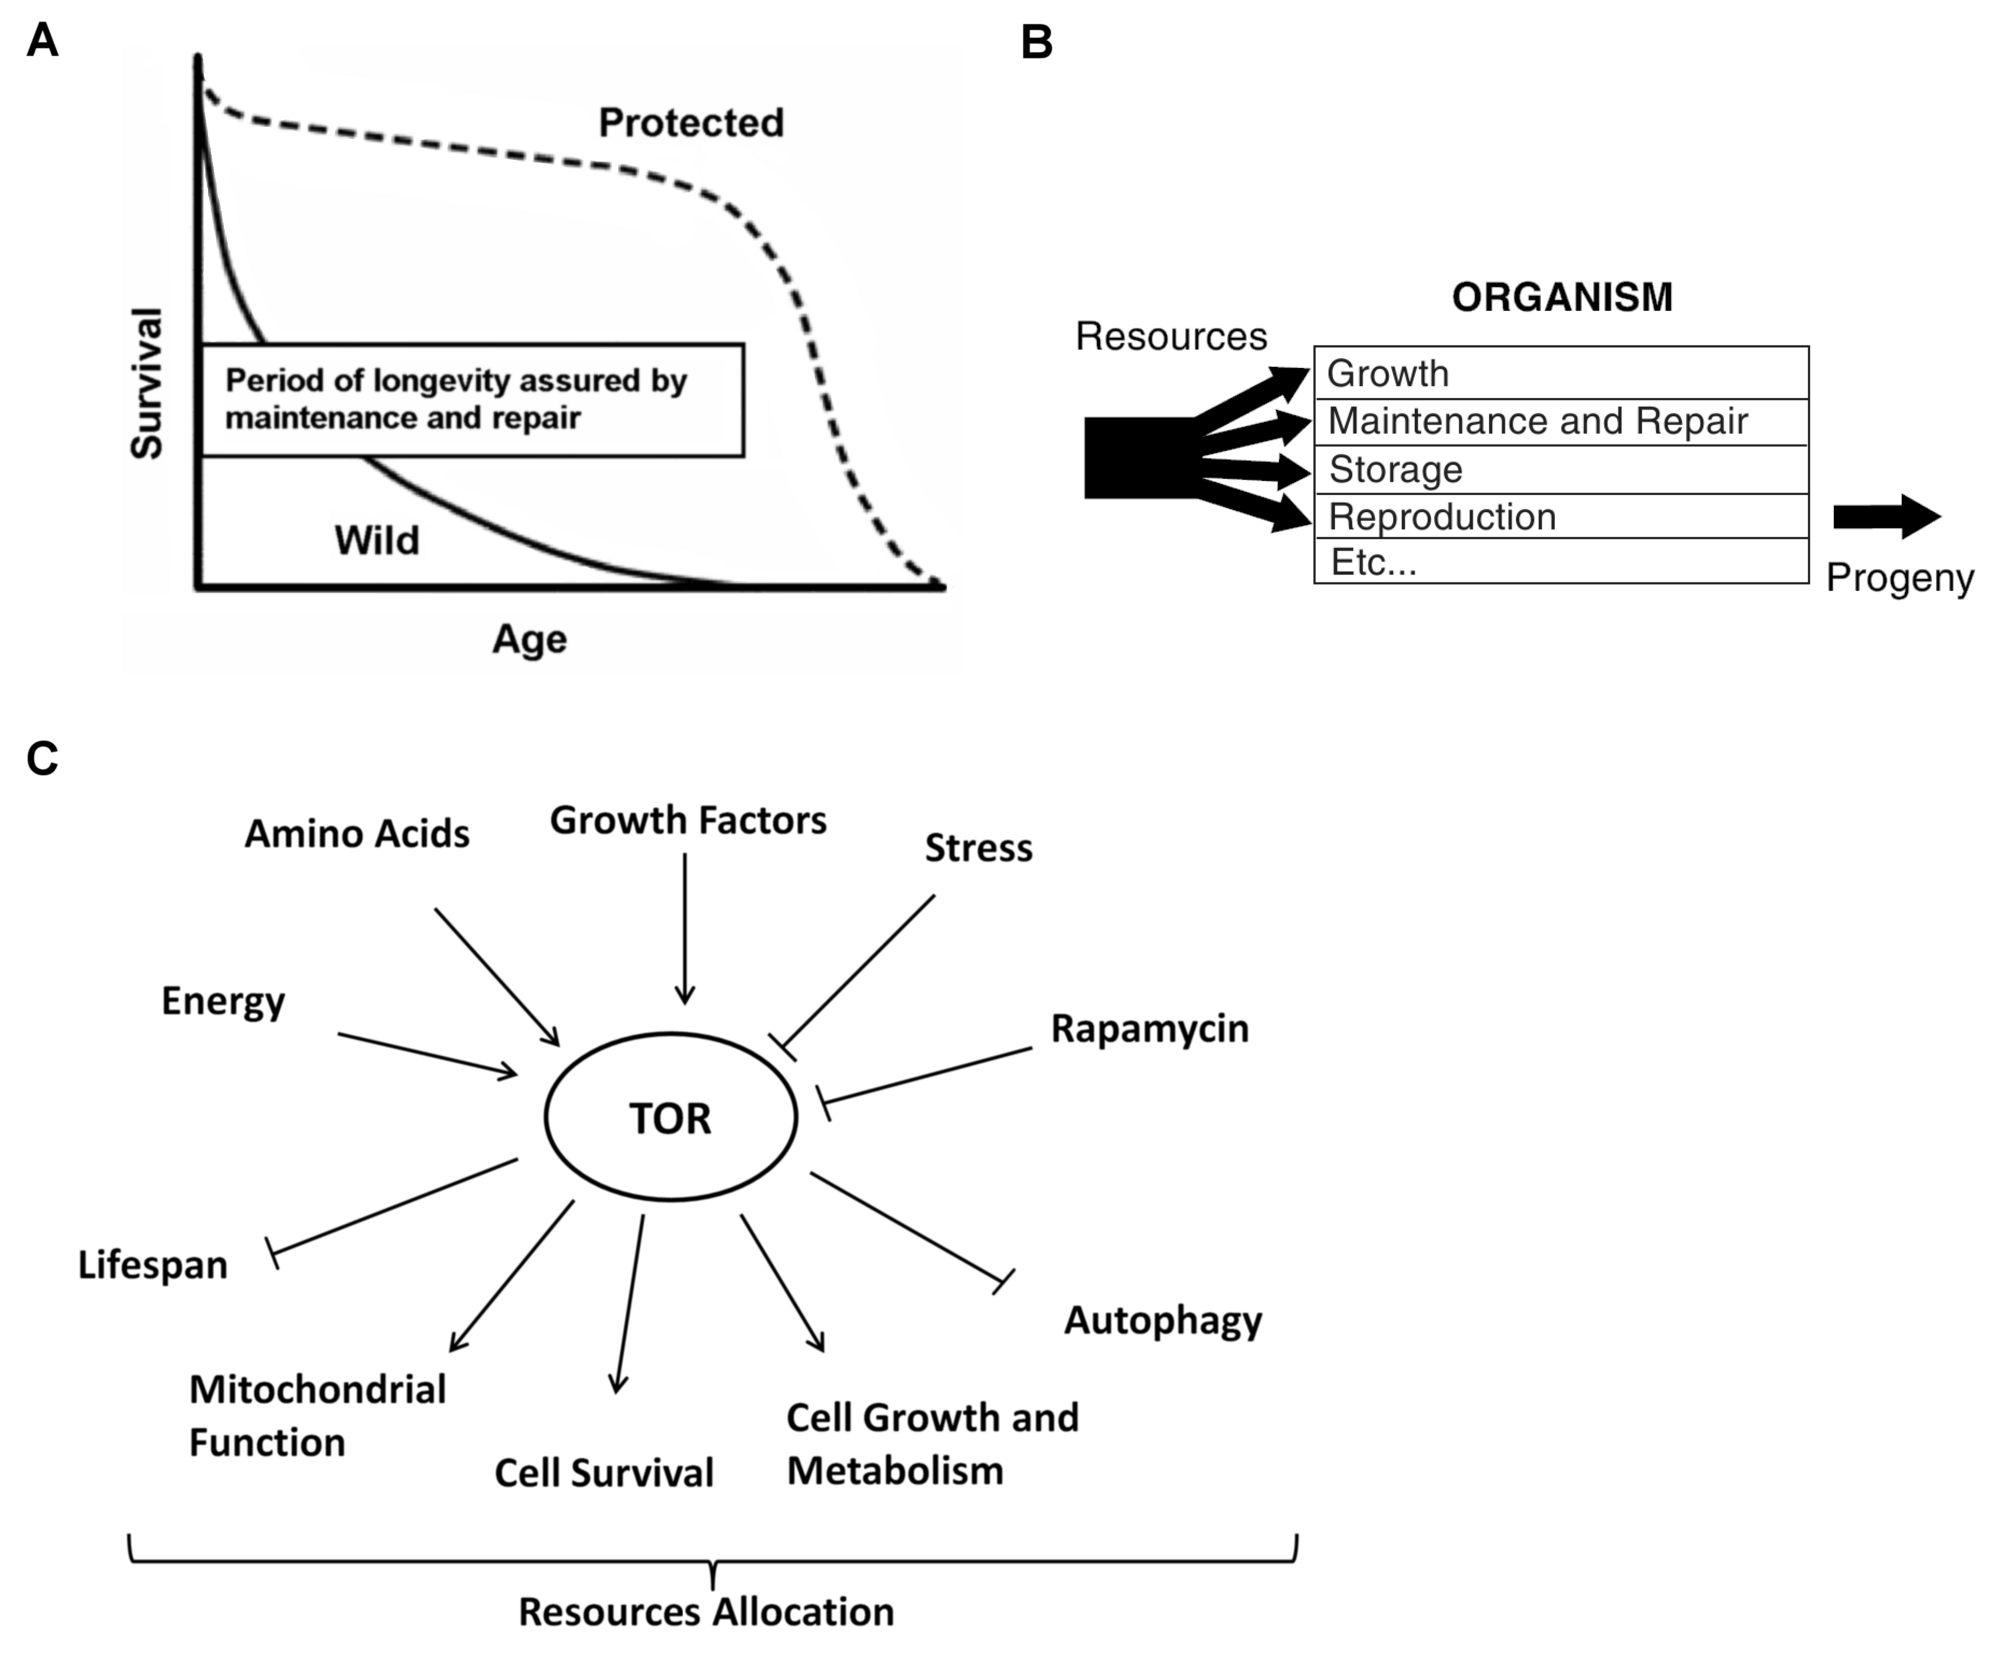
\includegraphics[width=5.6in]{dst_resalloc_tor.png}
		\caption[Disposable soma theory, resource allocation and TOR]{Disposable soma theory, resource allocation and TOR. (A) Lifespan differences between wild and protected environments. Adapted from \citep[Fig. 1]{Kirkwood2008}. (B) Resources allocation in the disposable soma theory of ageing \citep{Kirkwood1977, Kirkwood1981,Kirkwood2008}. In this theory, the problem of resource allocation is crucial since resources are limited and maintenance is costly. Adapted from \citep[Fig. 3]{Kirkwood2008}. (C) TOR in ageing. In response to stimuli such as insulin or growth factors, amino acids, energy and stress, Target of Rapamycin (TOR) kinase governs numerous age-related cellular processes regulating the allocation of resources.}
		\label{fig:dst_resalloc_tor}
	\end{center}
\end{figure}

\clearpage

\begin{figure}[tb]
	\begin{center}
		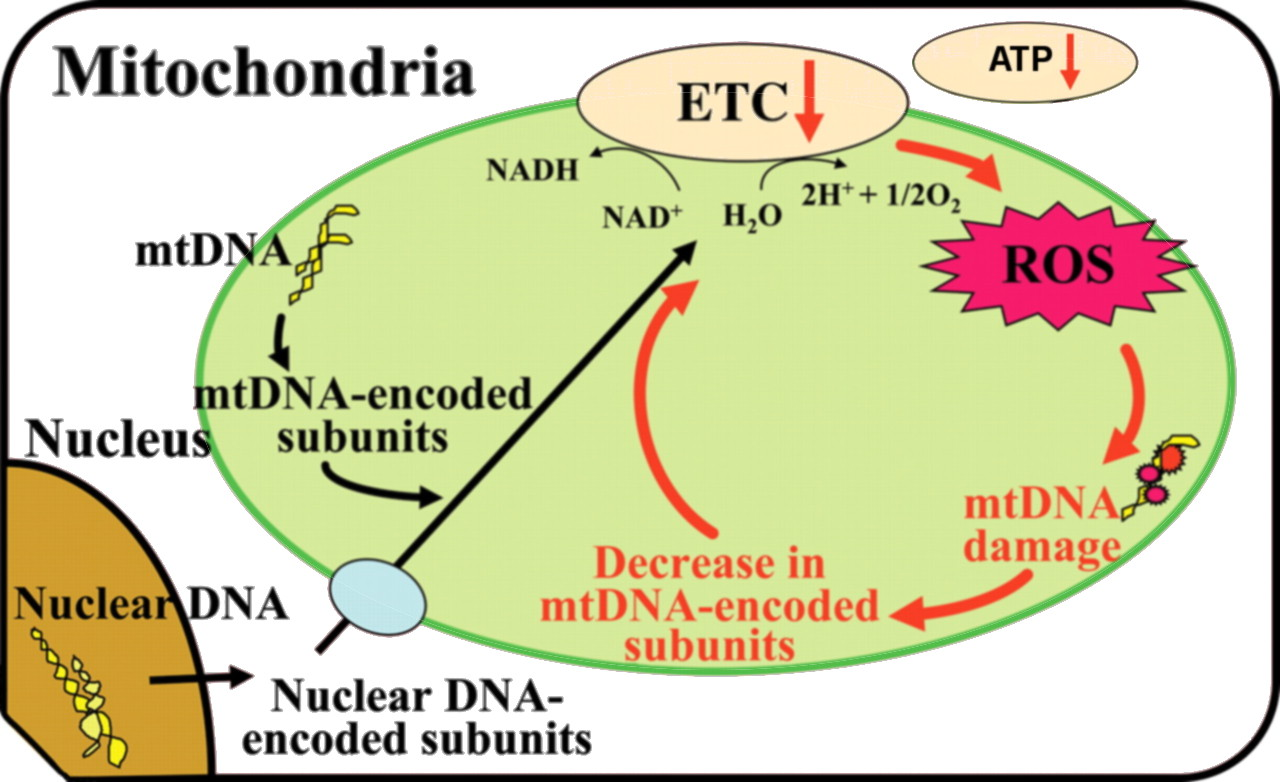
\includegraphics[width=3in]{Tsutsui09_fig1_adapted.jpg}
		\caption[ROS production and mitochondrial dysfunction]{ROS production and mitochondrial dysfunction. Mitochondrial DNA (mtDNA) in combination with nuclear DNA encode proteins building the mitochondrial electron transport chain (ETC), whose activity can be measured by mitochondrial membrane potential. Through ETC, molecules of adenosine triphosphate (ATP) are synthesised and utilised by the cell as an energy supply. Aside from ATP production, mitochondrial ETC also produces reactive oxygen species (ROS) as a waste product. ROS accumulation, due to a lack of ROS detoxification, severely damages mtDNA subunits, establishing a vicious circle which decreases mitochondrial function, energy levels within the cell, and increases ROS production and mutated mtDNA. Adapted from \citep[Fig. 1]{Tsutsui2009}.}
		\label{fig:Tsutsui09_fig1_adapted}
	\end{center}
\end{figure}

\clearpage




% ------------------------------------------------------------------------


%%% Local Variables: 
%%% mode: latex
%%% TeX-master: "../thesis"
%%% End: 
